Let x,y be two numbers
Given
\begin{align}
  x+y=24\\
  \implies y=24-x
\end{align}
For their product to be maximum
\begin{align}
    f(x)=xy=x(24-x)=24x-x^2 \label{aug/2/4/eq:1}
\end{align}
\begin{lemma}
A function f(x) is said to be concave if following inequality is true for $\lambda \in [0,1] :$  \label{aug/2/4/lemma1}
\begin{align}
    \lambda f(x_1) + (1-\lambda)f(x_2) \leq f(\lambda x_1 + (1-\lambda)x_2)
\end{align}
\end{lemma}
Checking convexity of $f(x)$ :
\begin{align}
    &\lambda(24{x_1}-{x_1}^2) + 
    (1-\lambda)\brak{24 {x_2}- {x_2}^2} \\ &\leq
    24(\lambda x_1 + (1-\lambda)x_2)-\brak{\lambda x_1 + (1-\lambda)x_2}^2 
\end{align}
\begin{align}
    \lambda(\lambda - 1)({x_1} -{x_2})^2 &\leq 0\\
    \implies \lambda(\lambda - 1)&\leq 0
\end{align}is true .
$\implies$
The function is concave.
Using gradient ascent method we can find its maxima,
    \begin{align}
        x_{n+1} &= x_n + \alpha \nabla f(x_n) \\
        \implies x_{n+1} &= x_n + \alpha \brak{-2x_n+24}
    \end{align}
    
    Taking $x_0=2,\alpha=0.001$ and precision= \\ 0.00000001,values obtained using python are:
    \begin{align}
        \boxed{\text{Maxima} =143.9999999999752 \approx 144 }\\
        \boxed{\text{Maxima Point} =  11.999995019260913\approx 12}
    \end{align}
We can verify this by the derivative test.
Since $f(x)$ is a concave function it has a maxima.
\begin{align}
\frac{df(x)}{dx}=-2x+24
\end{align}
Critical point :
\begin{align}
 \frac{df(x)}{dx}&=0\\
 -2x+24&=0\\
 x&=12
\end{align} 
is a critical point.And since $f(x)$ is a concave function there will be a maxima at $x=12$.
And the maxima is
\begin{align}
f(12)&=144
\end{align}
%
\begin{figure}[!h]
    \centering
    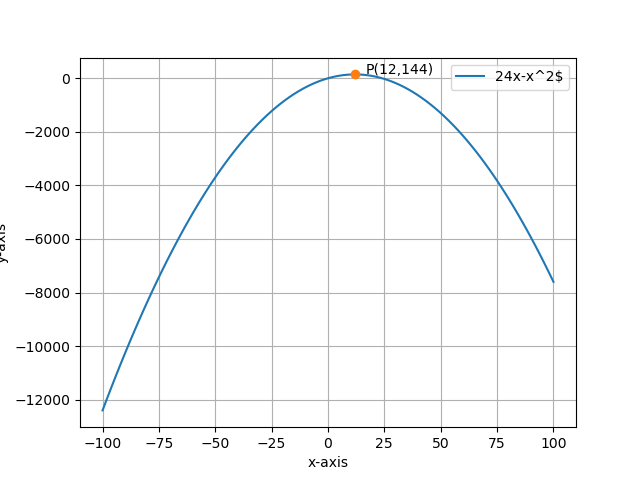
\includegraphics [width=\columnwidth]{solutions/aug/2/4/assignment6.png}
    \caption{$f(x)=24x-x^2$}
    \label{aug/2/4/p(x)}	
\end{figure}
